\documentclass[12pt]{article}%
\usepackage{amsfonts}
\usepackage{fancyhdr}
\usepackage{comment}
\usepackage[a4paper, top=2.5cm, bottom=2.5cm, left=2.2cm, right=2.2cm]%
{geometry}
\usepackage{times}
\usepackage{amsmath}
\usepackage{changepage}
\usepackage{amssymb}
\usepackage{graphicx}%
\usepackage{lipsum}
\usepackage{array}
\usepackage{listings}
\usepackage{color}
\usepackage{xcolor}

\delimitershortfall-1sp
\newcommand\abs[1]{\left|#1\right|}
\graphicspath{ {./images/} }

\definecolor{lightgray}{RGB}{214, 219, 223}
\definecolor{limegreen}{RGB}{11, 83, 69}
\definecolor{blue}{RGB}{0, 70, 255}
\lstdefinestyle{mystyle}{
    backgroundcolor=\color{lightgray},   
    commentstyle=\color{limegreen},
    keywordstyle=\color{blue}
}
 
\lstset{style=mystyle}
\makeatletter
\renewcommand{\maketitle}{\bgroup\setlength{\parindent}{0pt}
\begin{flushleft}
  \textbf{\@title}

  \@author
  \@date
\end{flushleft}\egroup
}
\makeatother


\begin{document}

\title{Weekly Assignment 2}
\author{Leong Kai Ler \\ 15334636 \\   }
\date{February 6, 2019}
\maketitle

\section*{Question 1}
A 6-sided die is rolled three times.
 
\subsection*{Problem part a}
How many elements are there in the same space ?
\subsection*{Solution part a}
A dice has 6 possible values. Rolling it 
Sample space S=\{(1,1,1), (1,1,2),  (1,1,3), ... (6,6,1), (6,6,2), ...(6,6,6)\}, so \begin{math} \abs{S}=6^3=216 \end{math} elements.
\subsection*{Problem part b}
Out of the possible sets of outcomes, calculate in how many at one least 2 rolled. \\
Using this, calculate what the probability is that at least one 2 is rolled.
\subsection*{Solution part b}
There are \begin{math} \frac{5}{6} \end{math} chance not getting 2 from a rolled dice. When the dice is rolled 3 times, the chance not getting any 2 is \begin{math}(\frac{5}{6})^3 \end{math}. So, to calculate the probability of getting at least one 2, we can subtract the probability of not getting any 2 from 1, hence 
\begin{equation*}
1 - (\frac{5}{6})^3 = \frac{91}{216	} \approx 0.4213
\end{equation*}
\newpage
\subsection*{Problem part c}
Write a small matlab simulation of this experiment and confirm that the observed
probability that at least one 2 is rolled matches your calculation in (a).
\subsection*{Solution part c}
\lstinputlisting[language=Matlab]{./matlab/weekly_assignment2_q1c.m} 
Result: \\
\begin{center}
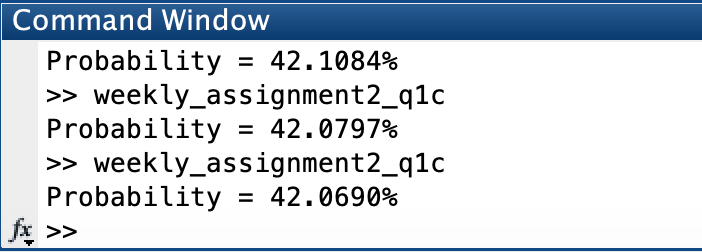
\includegraphics[scale=0.8]{q1c_result} \\
\end{center} 
The results obtained from the 1 million simulations is slightly higher($\pm0.2\%$) than the calculated result from 1b.
\newpage
\subsection*{Problem part d}
What is the probability that the sum of the die rolls is 17 ?
\subsection*{Solution part d}
The highest sum the dice rolls can get is 18, i.e \begin{math}6+6+6=18\end{math}. This means to get a sum of exactly 17, at least two dice have to produce 6, while the third dice rolled produce a 5. Hence,
\begin{equation*}
S=\{(1,1,1), (1,1,2),  (1,1,3), ... (6,6,1), (6,6,2), ...(6,6,6)\} 
\end{equation*} 
Let $E$ be the event where the sum of dice rolls is 17.
\begin{equation*}
E=\{(5,6,6),(6,5,6),(6,6,5)\}
\end{equation*}
\begin{equation*}
P(E)= \frac{\abs{E}}{\abs{S}} = \frac{3}{216} \approx 0.0139
\end{equation*}

\subsection*{Problem part e}
What is the probability that the sum of the three dice rolls is 12 given that the first roll was a 1 ?
\subsection*{Solution part e}
Since it's not a conditional probability, we can just take into account of the sum of two subsequent dice rolls instead of three. That being said let E be the event where the subsequent two dices rolled sums up to $12 - 1 = 11$. 
\begin{eqnarray*}
S & = &\{(1,1), (1,2),  (1,3), ... (6,1), (6,2), ...(6,6)\} \\
\abs{S} & = & 6^2 = 36 \\ \\
E & = & \{(5,6),(6,5)\} \\
\abs{E} & = & 2 \\ 
P(E) & = & \frac{\abs{E}}{\abs{S}} \\
	 & = & \frac{2}{36} \\
	 & \approx & 0.0556 \\
\end{eqnarray*}



\newpage
\section*{Question 2}
I roll a 6-sided die. If it comes up a 1 then I throw a six-sided die and otherwise a 20-sided die.
\subsection*{Problem part a}
What is the probability that the second throw comes up a 5 ?
\subsection*{Solution part a}
Split the calculation into 2 cases. 
\begin{itemize}
\item rolling a 6 sided dice: \\ There is a $\frac{1}{6}$chance of rolling a 6 sided dice after the first dice rolled. From there, there is another $\frac{1}{6}$ chance of getting a 5. Hence, $\frac{1}{6} * \frac{1}{6} = \frac{1}{36}$
\item rolling a 20 sided dice: \\ There is a $\frac{5}{6}$chance of rolling a 20 sided dice after the first dice rolled. From there, there is another $\frac{1}{20}$ chance of getting a 5. Hence, $\frac{5}{6} * \frac{1}{20} = \frac{1}{24}$
\end{itemize}
So, probability that the second throw comes up a 5 is $\frac{1}{36}+\frac{1}{24}=\frac{5}{72}\approx 0.0694$
\subsection*{Problem part b}
What is the probability that the second throw comes up a 15? \\ Hint: use marginalisation
\subsection*{Solution part b}
It is impossible to get a 15 from a six sided dice in the second throw. Hence, we skip to probability of getting a 15 from a 20 sided dice in the second throw. \\ \\
Let $F_i$ be the event of getting i values from first dice rolled and E be the event of getting 15 in the second throw.
\begin{center}
\begin{tabular}{|| p{4cm} | c | c | c | c | c | c ||}
\hline
Possible values from first throw & 1 & 2 & 3 & 4 & 5 & 6 \\
\hline\hline 
Probability of getting 15 in second throw & 0 & $\frac{1}{20}$ & $\frac{1}{20}$ & $\frac{1}{20}$ & $\frac{1}{20}$ & $\frac{1}{20}$ \\
\hline
\end{tabular}
\end{center}
\begin{eqnarray*}
P(E) & = & P(E \cap F_1 ) + P(E \cap F_2 ) + \cdot \cdot \cdot + P(E \cap F_n ) \\
	 & = & 0 + \frac{1}{6} * \frac{1}{20} + \frac{1}{6} * \frac{1}{20} + \frac{1}{6} * \frac{1}{20} + \frac{1}{6} * \frac{1}{20} + \frac{1}{6} * \frac{1}{20} \\
	 & = & 0 + \frac{5}{6} * \frac{1}{20} \\
	 & = & \frac{1}{24} \\
	 & \approx & 0.0417
\end{eqnarray*}

\newpage
\section*{Question 3}
At a certain stage of a criminal investigation, the inspector in charge is 60 percent convinced of the guilt of a certain suspect. Suppose, however, that a new piece of evidence which shows that the criminal has a certain characteristic (such as left- handedness, baldness, or brown hair) is uncovered. If 20 percent of the population possesses this characteristic, use Bayes Rule to calculate how certain of the guilt of the suspect should the inspector now be if it turns out that the suspect has the characteristic. \\
\subsection*{Solution:}
Let 
\begin{itemize}
\item $P(E|F) =$ Probability of being criminal given the specific characteristic
\item $P(E) =$ Probability of being criminal $= 0.6$
\item $P(F|E) =$ Probability of having characteristic given being criminal $= 1.0$
\item 
	$P(F) = $ Probability of having brown hair  
\end{itemize}
\begin{eqnarray*}
P(F) & = & P(F|E) * P(E) + P(F|E^c) * P(E^c) \\
	 & = & 1.0 * 0.6 + 0.2 * 0.4 \\
	 & = & 0.68 \\ \\
P(E|F) & = & \frac{P(F|E) * P(E)}{P(F)} \\
	   & = & \frac{1.0 * 0.6}{0.68} \\
	   & = & \frac{15}{17} \\
	   & \approx & 0.882 \\
\end{eqnarray*} 
Inspector should now be 0.882 certain of the guilt of the suspect if it turns out that the suspect has the characteristic.
\newpage
\section*{Question 4}
Your cell phone is constantly trying to keep track of where you are. At any given point in time, for all nearby locations, your phone stores a probability that you are in that location. Right now your phone believes that you are in one of 16 different locations arranged in a grid with the following probabilities (see the figure on the left):

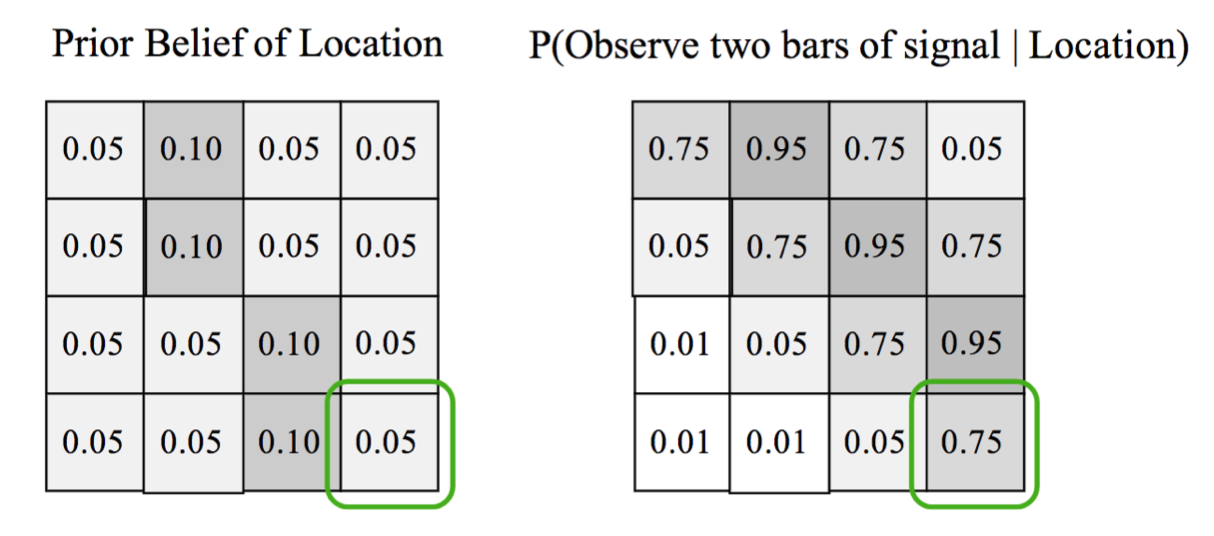
\includegraphics[scale=0.7]{figure}

Your phone connects to a known cell tower and records two bars of signal. For each grid location L you know the probability of observing two bars from this particular tower, given that the cell phone is in location L (see the figure on the right). Example: the highlighted cell on the left figure means that you believed there was a 0.05 probability that the user was in the bottom right grid cell prior to observing the cell tower signal. The highlighted cell on the right figure means that you think the probability of observing two bars, given the user was in the bottom right grid cell, is 0.75.
\\ \\
For each of the 16 location positions, calculate the new probability that the user is in each location given the cell tower observation. Write a program to calculate the probabilities. Report the probabilities of all 16 cells and write a short explanation of your program.
\newpage
\subsection*{Solution:}
Let 
\begin{itemize}
\item $P(L) = $ Prior Belief of Location
\item $P(O|L) = $ Probability of observing two bars from a signal given the location L
\item $P(O) = $ Tower Signal
\item $P(L|O) = $ Probability of Location given the observation \\
\end{itemize} 
Since $P(L)$ and $P(O|L)$ are given, we only need to calculate $P(O)$ to compute $P(L|O)$ for each cell.
\begin{eqnarray*}
P(O) & = & P(O|L) * P(L) + P(O|L^c) * P(L^c)\\
	 & = & P(O|L) * P(L) + P(O \cap L^c) \\
P(L|O) & = &\frac{P(O|L)*P(L)}{P(O)} \\
	   & = &\frac{P(O|L)*P(L)}{P(O|L) * P(L) + P(O \cap L^c)} \\
\end{eqnarray*} \\
Take an example with the marked cell in row 4 and column 4, in the figure above, we can calculate its corresponding $P(O)_{44}$ using marginalisation and $P(L|O)_{44}$ using the formula above. 
\begin{eqnarray*}
P(O \cap L^c)_{44} & = & P(O \cap L^c)_{00} + P(O \cap L^c)_{01} + \cdots + P(O \cap L^c)_{43} \\
& = & 0.05 * 0.75 + 0.10 * 0.95 + \cdots + 0.10 * 0.05 \\
& = & 0.4665 \\
P(O)_{44} & = & P(O|L)_{44} * P(L)_{44} + P(O \cap L^c)_{44} \\
	 & = & 0.75 * 0.05 + 0.4665 \\
	 & = & 0.504 \\ \\
P(L|O)_{44} & = &\frac{P(O|L)_{44}*P(L)_{44}}{P(O)_{44}} \\
	   & = &\frac{P(O|L)_{44}*P(L)_{44}}{P(O|L)_{44} * P(L)_{44} + P(O \cap L^c)_{44}} \\
	   & = &\frac{0.75 * 0.05}{0.504} \\
	   & = &\frac{25}{336} \\
	   & \approx & 0.0744	  
\end{eqnarray*} 
Finally, using the following code, we can compute $P(L|O)$ based for every cell on the method shown above. 
\newpage
\subsection*{Code:}
\lstinputlisting[language=Matlab]{./matlab/weekly_assignment2_q4.m}
\newpage
\subsection*{Results:}
Probabilities of all 16 cells computed: \\
Array form: \\
\begin{center}
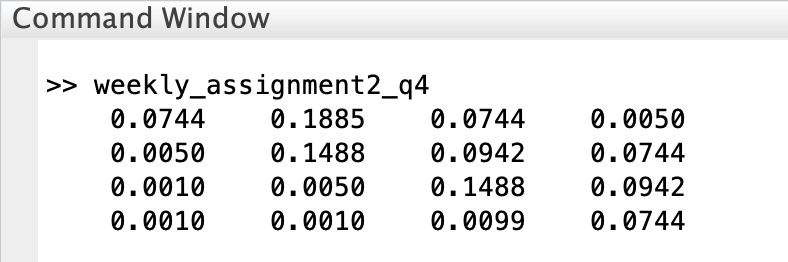
\includegraphics[scale=0.8]{q4_result} \\
\end{center}
Tabular form: \\
\begin{center}
\begin{tabular}{| c | c | c | c |}
\hline
0.0744 & 0.1885 & 0.0744 & 0.0050 \\
\hline
0.0050 & 0.1488 & 0.0942 & 0.0744 \\
\hline 
0.0010 & 0.0050 & 0.1488 & 0.0942 \\
\hline
0.0010 & 0.0010 & 0.0099 & 0.0744 \\
\hline
\end{tabular}
\end{center}
\end{document}